%newpage here since motivation usualy starts on page3
\newpage
\section{Motivation and Background}
\label{background}

Motivate moore's law slowing, we want continuous performance scalability, etc.

About transparency. Multi-GPU systems are here but besides HPC (maybe graphics 
as well) which knows how to use them efficiently (MPI process per GPU), the rest 
of the market needs to re-think, re-write, and re-compile its code. We advocate 
for the runtime which allows a kernel to be partitioned into sub-kernels and 
distributes each of them to a different GPU device. In the future, the number of 
GPUs and inter-GPU network complexity is going to increase, so we need to hide 
that from a programmer.
Problems of NUMA systems are well known in CPU world. Remote traffic is a 
problem which can be solved either with some dynamic memory page allocation 
policy (migrations and replications) or NUMA-aware thread scheduling. We focus 
on the architectural tweaks.


Chart supports the fact that we have plenty of CTAs to fill a multi-GPU without a problem
and that our memory footprints are big enough to not be cache resident in this study.

\begin{table}[t]
\begin{small}
\centering
\begin{tabular}{lccc}
 \toprule
 \textbf{Benchmark} & \textbf{Kernels} & \textbf{Time-weighted} & \textbf{Memory} \\
& & \textbf{Average CTAs} & \textbf{Footprint (MB)} \\
 \toprule
ML-GoogLeNet-cudnn-L2 & 1 & 6272.0 & 1204.7 \\
ML-AlexNet-cudnn-L2 & 1 & 1250.0 & 832.4 \\
Optix-Raytracing & 1 & 3072.0 & 86.7 \\
Bitcoin-Crypto & 1 & 60.0 & 5898.2 \\
ML-OverFeat-cudann-L3 & 1 & 1800.0 & 387.5 \\
Encription & 1 & 128.0 & 0.8 \\
ML-AlexNet-cudnn-L4 & 1 & 1014.0 & 32.4 \\
ML-AlexNet-ConvNet2 & 1 & 6075.0 & 97.2 \\
HPC-Namd2.9 & 1 & 3888.0 & 88.3 \\
HPC-RabbitCT & 1 & 131072.0 & 524.3 \\
Rodinia-Backprop & 2 & 4096.0 & 160.2 \\
Rodinia-Euler3D & 346 & 1008.0 & 25.2 \\
Rodinia-BFS & 24 & 1954.0 & 38.5 \\
Rodinia-Gaussian & 510 & 2599.1 & 78.0 \\
Rodinia-Hotspot & 1 & 7396.0 & 63.9 \\
Rodinia-Kmeans & 3 & 3249.0 & 220.8 \\
Rodnia-Pathfinder & 20 & 4630.0 & 1570.0 \\
Rodinia-Srad & 4 & 16384.0 & 98.4 \\
Lonestar-SP & 11 & 75.0 & 7.6 \\
HPC-Lulesh & 105 & 12202.1 & 577.6 \\
Lonestar-MST-graph & 87 & 770.1 & 85.9 \\
Lonestar-MST-mesh & 71 & 894.6 & 74.8 \\
HPC-CoMD & 350 & 3588.5 & 318.6 \\
HPC-CoMD-wa & 350 & 13691.2 & 392.8 \\
HPC-CoMD-ta & 350 & 5724.0 & 393.9 \\
HPC-HPGMG-UVM-opt & 359 & 10436.5 & 1975.5 \\
HPC-HPGMG & 317 & 10506.4 & 1571.5 \\
HPC-HPGMG-UVM-base & 359 & 10727.8 & 1975.5 \\
HPC-Lulesh-Unstruct-small & 2000 & 434.9 & 18.7 \\
HPC-Nekbone-medium & 510 & 3093.4 & 170.0 \\
Lonestar-SSSP-wln & 1000 & 60.2 & 20.5 \\
HPC-SNAP & 118 & 200.2 & 744.1 \\
HPC-Nekbone-large & 300 & 5582.7 & 294.0 \\
HPC-MiniAMR & 33 & 76033.1 & 2751.7 \\
HPC-MiniContact-large & 127 & 15423.2 & 257.2 \\
HPC-MiniContact-small & 500 & 250.4 & 20.8 \\
HPC-Lulesh-Unstruct-large & 200 & 4939.9 & 208.1 \\
HPC-AMG & 88 & 241548.9 & 3743.9 \\
HPC-RSBench & 1 & 7813.0 & 19.1 \\
HPC-MCB & 1 & 5001.0 & 161.8 \\
Lonestar-DMR & 3 & 82.1 & 247.9 \\
Lonestar-SSSP-wlc & 1300 & 163.3 & 21.2 \\
Lonestar-SSSP & 102 & 1046.0 & 38.2 \\
Stream-Triad & 5 & 699051.0 & 3145.7 \\
\toprule
\end{tabular}
\caption{Number of CTAs and total memory footprint when compared to multi-socket GPU with 256 active CTA contexts containing XXX MB of LLC.}
\label{tab:numctas}
\end{small}
\end{table}



\subsection{A Multi-Socket GPU Runtime}

As demonstrated by Cabezas et al.~\cite{Cabezas2015} it is possible to design 
a framework and a runtime system that transparently decomposes GPU kernels in 
sub-kernels and executes them on multiple GPUs in parallel. On the Nvidia 
GPUs, this is doable by intercepting and remapping each single kernel call, 
GPU memory allocation, GPU memory copy and GPU wide synchronization issued by 
the CUDA driver. Special care needs to be put (i) to the GPU local memory 
fences which needs to be promoted to system level and (ii) to the the 
sub-kernels CTA identifiers which needs to be properly recomputed to 
reflect those in the original kernel call. 
 
In ~\cite{Cabezas2015} these two problems were solved by introducing custom 
code annotations and an additional source-to-source compiler which was also 
responsible for statically assigning data and computation on each GPU. In our 
work, we follow a very similar strategy but we do not use any additional 
compiler for two reasons (i) we use a simulated environment in which 
we can properly modify the architecture to account for required memory fences 
and sub-kernel to kernel CTA identifiers mapping (ii) we model a system in 
which all GPU memory allocations are performed on system memory, explicit 
CUDA memory copies are disabled and we use the recently introduced feature to 
migrate pages on demand at first touch (FT) using the UVM page faulting 
mechanism~\cite{P100}. 

With respect to data placement, while on a single GPU interleaving memory at 
the granularity of single cache line is routinely done to reduce memory 
camping effects and maximize bandwidth, doing it across multiple GPUs 
disrupts locality and results in large amount of remote accesses even for 
regular and dense applications. A middle ground alternative between first 
touch page allocation and static fine grain cache line interleaving is to 
perform page granularity interleaving across the various GPU memories.

While on a single GPU, round-robin fine grain assignment of CTAs to the SMs 
to achieve perfect load balancing is standard, extending this on a Multi-GPU 
system does not make much sense. For start, the cost of launching a kernel on 
a single GPU is in the order of 10 micro seconds, so trying to create large 
amount of sub-kernels of the size of a few CTAs results in huge overheads. 
For this reason as in~\cite{Cabezas2015}, we decompose a single kernel in N 
sub-kernels (where N is the total number of GPUs in the system) and we assign 
to each GPU an equal amount of contiguous CTAs. The danger of this approach 
is to expose workload unbalance in the CTAs. This can be reduced by selecting 
the CTAs in each sub-kernel to be non contiguous, for instance sending to 
each GPU the CTAs which identifiers modulo the GPU identifier are zero or 
randomly selecting them. However, selecting CTAs in not contiguous fashion
also disrupts locality present in many dense and regular applications where 
contiguous CTAs, access contiguous memory.

In general the problems of data placement and task placement (minimizing 
remote data access and ensuring perfect load balancing) can not be completely 
decoupled. We found that first touch page placement and contiguous CTA 
assignment to be the best choice across our benchmark suites, again because it 
preserves locality when present. We will therefore use this as the baseline 
architecture for our studies in the rest of this paper.

Figure~\ref{fig:motivation2} quantitatively shows the reason behind our 
choice. We can clearly see that the speedup with respect to a single GPU 
(composed of 64 SM and with 768 GB/sec of memory bandwidth) achievable by a 4 
GPU system connected with NVLink at 128 GB/sec is much higher for the choice 
``contiguous CTA scheduling + FT page placement''. A more detailed 
description of the methodology and simulation parameters is in 
Section~\ref{methodology}. 
Also in Figure, for each application, we show the maximum  performance 
achievable by an hypothetically single GPU with 4x number of SMs and 4x 
memory bandwidth (red mark in Figure~\ref{fig:motivation2}). This mark 
represents a good approximation of the 
maximum theoretical performance we could expect for a perfect 4 GPU system. 
As we can see for some applications (on the right side of the graph) the 4 
GPU system with ``contiguous CTA scheduling + FT page placement'' already 
performs as good or better (in situations where larger cache capacity enables 
super scaling) than an hypothetical 4x larger single GPU. For other 
applications (on the left side of the graph) the gap between the red mark and 
what we can achieve with the baseline multi-GPU system is quite large. In the 
rest of this paper we present techniques aimed to reduce this gap. 
We want to stress the red mark in Figure~\ref{fig:motivation2} represents an 
upper bound and that a single GPU with 4x number of SMs and 4x bandwidth of 
the largest existing GPU is impossible without changing underline silicon 
technology. 




% \begin{figure}[tp]
%     \centering
%     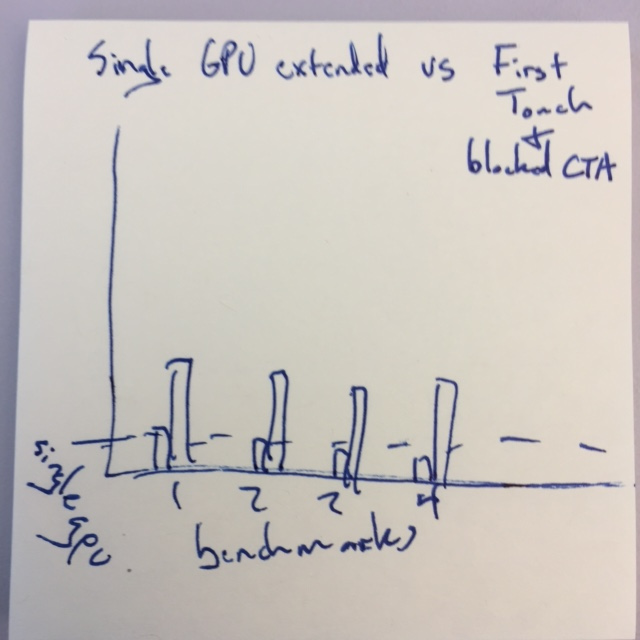
\includegraphics[width=0.9\columnwidth]{figures/motivation1.jpg}
%     \caption{Multi-socket GPU performance by applying known CPU NUMA localization techniques for scheduling and memory placement.}
%     \label{fig:motivation}
% \end{figure}

%Second figure now shows our baseline we're going to compare against - for %some benchmarks we can't expect speedup, its quite good already.
%For others there is a long ways to go and we're going to try and close that %gap now.

\begin{figure*}[tp]
    \centering
    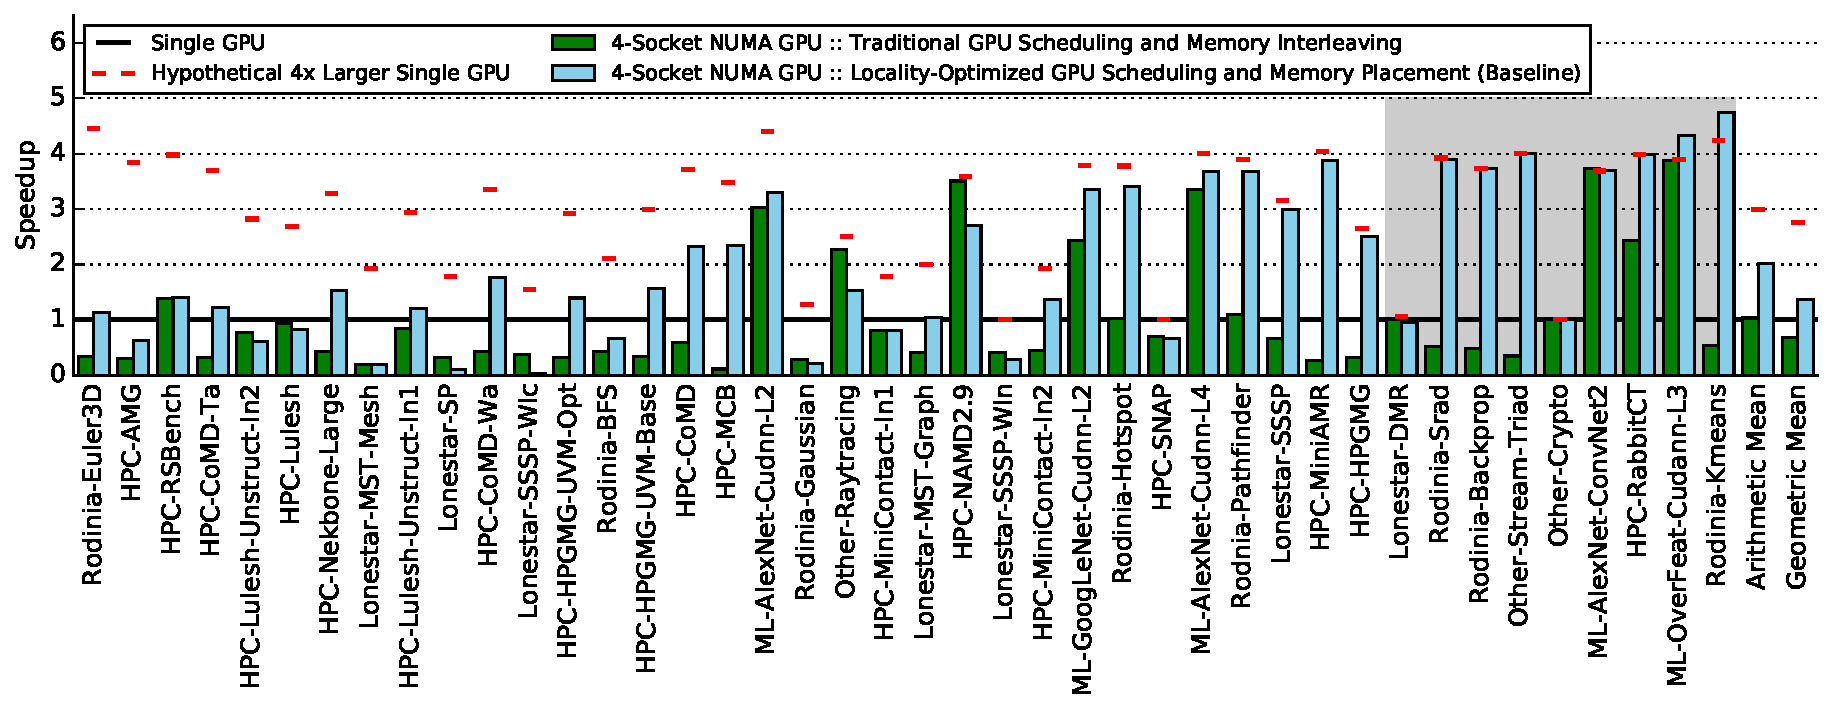
\includegraphics[width=1\linewidth]{figures/plot_different_baselines.pdf}
    \caption{Relative performance of multi-socket GPU to an unbuildable 4x larger GPU.}
    \label{fig:motivation2}
\end{figure*}

\subsection{Related Work}

This is going to come up front in this paper because there is a a bunch and we want to explain how
why this paper is different.

Multi-GPU work
Cache partitioning work
We do not optimize for latency (the highest hit rate) but for bandwidth (the hit rate is not the highest; we can show some graph later to support that the best cache configuration does not provide the highest hit rate)
Not sure about NVLink/interconnection related work
Discuss simplex vs duplex interconnects / point-to-point links
At least mention which interconnects / point to point links can have reversible links vs statically partitioned links (Ethernet, Infiniband, QPI)
Is there a reference that says that GRS signal links can reverse direction?


% Heterogeneous CPU--GPU systems have been widely
% adopted by the high performance computing community 
% and are becoming increasingly common in other computing paradigms.  High performance GPUs have 
% developed into stand-alone PCIe-attached accelerators requiring explicit memory 
% management by the programmer to control data transfers into the GPU's 
% high-bandwidth locally attached memory. As GPUs have evolved, the onus of 
% explicit memory management has been addressed by providing a unified shared
% memory address space between the GPU and CPU~\cite{UVM,HSA}.  Whereas a single 
% unified virtual address space improves programmer productivity, discrete GPU and 
% CPU systems still have separate locally attached physical memories, optimized for 
% bandwidth and latency respectively. 
% 
% Managing the physical location of data, and guaranteeing that reads access 
% the most up-to-date copies of 
% data in a unified shared memory can be done through the use of page level 
% migration and protection. Such mechanisms move data at the OS page granularity between 
% physical memories~\cite{UVM}.  With the advent of non-PCIe high-bandwidth, low-latency
% CPU--GPU interconnects, the possibility of performing cache-line, rather than OS-page-granularity, accesses
% becomes feasible.  Without OS page protection
% mechanisms to support correctness guarantees, however,  the responsibility of coherence
% has typically fallen on hardware cache-coherence implementations.
% 
% \ignore{Managing the physical location and coherence guarantee of 
% data in a unified shared memory can be done through the use of page level 
% migration and protection, which moves data at the OS page granularity between 
% physical memories~\cite{UVM}.  With the advent of non-PCIe high bandwidth, low latency,
% CPU--GPU interconnects the possibility of performing cache-line based accesses,
% rather than OS page granularity, becomes feasible.  Without OS page protection
% mechanisms to support shared memory guarantees, however,  the responsibility of coherence
% has typically fallen on hardware cache-coherence implementations.}
% 
% \begin{table}[t]
% \begin{center}
% \begin{tabular}{ddd}
%  \hline
%  \multicolumn{1}{l}{Workload} &   \multicolumn{1}{c}{L1 Hit Rate (\%)}  &  \multicolumn{1}{c}{L2 Hit Rate (\%)}  \\
%  \hline
%  \hline
%  \multicolumn{1}{l}{backprop}  &   62.4  &   70.0\\
%  \hline
%  \multicolumn{1}{l}{bfs}  &   19.6  &   58.6  \\
%  \hline
%  \multicolumn{1}{l}{btree}  &   81.8  &   61.8  \\
%  \hline
%  \multicolumn{1}{l}{cns}  &   47.0  &   55.2  \\
%  \hline
%  \multicolumn{1}{l}{comd}  &   62.5  &   97.1  \\
%  \hline
%  \multicolumn{1}{l}{kmeans}  &   5.6  &   29.5  \\
%  \hline
%  \multicolumn{1}{l}{minife}  &   46.7  &   20.4  \\
%  \hline
%  \multicolumn{1}{l}{mummer}  &   60.0  &   30.0  \\
%  \hline
%  \multicolumn{1}{l}{needle}  &   7.0  &   55.7  \\
%  \hline
%  \multicolumn{1}{l}{pathfinder}  &   42.4  &   23.0  \\
%  \hline
%  \multicolumn{1}{l}{srad\_v1}  &   46.9  &   25.9  \\
%  \hline
%  \multicolumn{1}{l}{xsbench}  &   30.7  &   63.0  \\
%  \hline
%  \hline
%  \multicolumn{1}{l}{Arith Mean}  &   44.4  &   51.6  \\
% \hline
% \end{tabular}
% \caption{GPU L1 and L2 cache hit rates (average).}
% \label{tab:gpuhitrate}
% \end{center}
% \vspace{-.2in}
% \end{table}
% 
% \begin{figure*}[t]
%     \centering
%     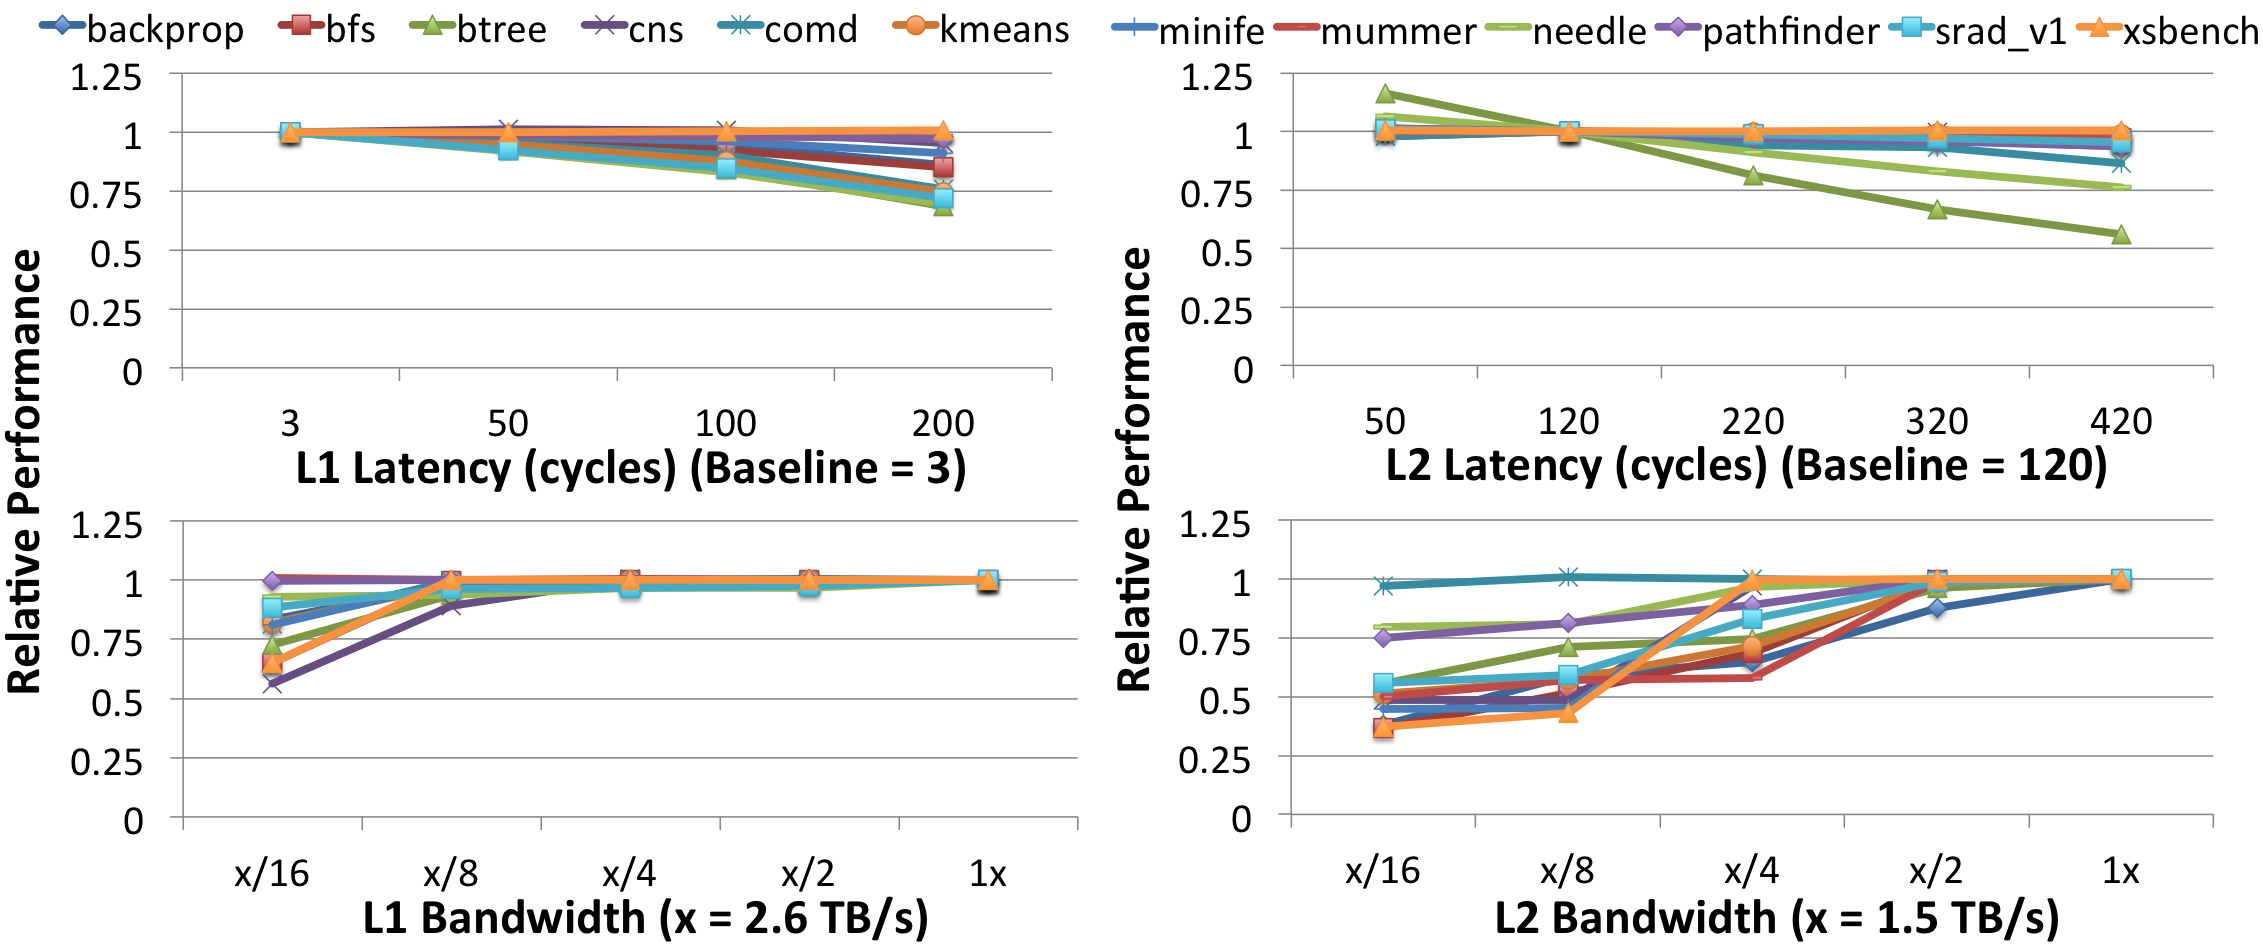
\includegraphics[width=0.9\textwidth]{figures/cache_bw_latency.png}
%     \caption{GPU performance sensitivity to L1 and L2 latency and bandwidth
% changes.}
%     \label{fig:cache_bw_latency}
%     \vspace{-.05in}
% \end{figure*}
% 
% As programming models supporting transparent CPU--GPU sharing become 
% more prevalent and sharing becomes more fine-grain and frequent, the 
% performance gap between page-level coherence and fine-grained hardware cache-coherent
% access will grow~\cite{Agarwal2015,Agarwal2015b,Lim2012}. 
% On-chip caches, and thus HW cache coherence, are widely used in CPUs because they 
% provide substantial memory bandwidth and latency 
% improvements~\cite{Martin2012}.
% Building scalable, high-performance cache coherence requires 
% a holistic system that strikes a balance between directory storage 
% overhead, cache probe bandwidth, and application 
% characteristics~\cite{Power2013,Pugsley2010,Cantin2005,johnson2011,Hong2012,Sanchez2012,Kelm2010}.
% Although relaxed or scoped consistency models allow coherence operations
% to be re-ordered or deferred, hiding latency, they do not obviate the need 
% for HW cache coherence. However, supporting a CPU-like HW coherence model
% in large GPUs, where many applications do not require coherence, is a tax on GPU designers.  Similarly,
% requiring CPUs to relax or change their HW coherence implementations or implement instructions
% enabling software management of the cache hierarchy adds significant system complexity.
% 
% Prior work has shown that due to their many threaded design, GPUs are 
% insensitive to off-package memory latency but very sensitive to off-chip memory 
% bandwidth~\cite{Agarwal2015,Agarwal2015b}. Table~\ref{tab:gpuhitrate}
% shows the L1 and L2 cache hit rates across a variety of workloads from the Rodinia 
% and United States Department of Energy application suites~\cite{Che2009,villa2014}.  These low hit 
% rates cause GPUs to also be fairly
% insensitive to small changes in L1 and L2 cache latency and bandwidth, as shown in 
% Figure~\ref{fig:cache_bw_latency}.  This lack of sensitivity raises the question whether GPUs need 
% to uniformly employ on-chip caching of all off-chip memory to achieve good performance.  If GPUs do not 
% need or can selectively employ on-chip caching, then CPU--GPU systems can be built that
% present a unified, coherent shared-memory address space to the CPU, while not requiring a 
% HW cache-coherence implementation within the GPU. 
% 
% Avoiding hardware cache coherence benefits GPUs by decoupling them from the coherence protocol 
% implemented within the CPU complex, enables simplified GPU designs, and improves
% compatibility across future systems. It also reduces the scaling load on the 
% existing CPU coherence and directory structures by eliminating the potential addition
% of hundreds of caches, all of which may be sharing data. However, selective caching does not come without
% a cost. Some portions of the global memory space will become un-cacheable
% within the GPU\@ and bypassing on-chip caches can place additional load 
% on limited off-chip memory resources.  In the following sections, we show that by leveraging
% memory request coalescing, small CPU-side caches, improved interconnect efficiency, and
% promiscuous read-only caching, selective caching GPUs can perform nearly as well
% as HW cache-coherent CPU--GPU\@ systems.
